% -*- coding: UTF-8 -*-
% vim: autoindent expandtab tabstop=4 sw=4 sts=4 filetype=tex
% vim: spelllang=de spell
% chktex-file 27 - disable warning about missing include files

\chapter{Theoretischer Hintergrund}
\label{chap:theoretical_background}

Sofern im Text nicht anders vermerkt, basiert das folgende Kapitel
auf~\cite[S. 721ff]{foley_computer_1996}.

Für die Erzeugung und Darstellung von Bildern werden zwei Angaben
benötigt: Was dargestellt werden soll und wie dieses dargestellt werden
soll.
Prinzipiell geht es darum zu bestimmen, welche Farbe eine Oberfläche an
einem bestimmten Punkt hat. Dabei haben sich die Begriffe des
\textit{Beleuchtungsmodelles (illumination model)} und des
\textit{Modelles zur Schattierung (shading model)} etabliert.

\citeauthor{foley_computer_1996} nutzt den Begriff \textit{shading model} als
Überbegriff, welcher auch Beleuchtungsmodelle umfasst. Daher definiert ein
\textit{shading model}, wann ein Beleuchtungsmodell mit welchen
Parametern angewendet wird. So nutzen manche \textit{shading models} ein
Beleuchtungsmodell für jeden Pixel, andere wiederum nur für einzelne Pixel und
interpolieren dabei die Werte der anderen Pixel.

% -*- coding: UTF-8 -*-
% vim: autoindent expandtab tabstop=4 sw=4 sts=4 filetype=tex
% chktex-file 27 - disable warning about missing include files

\section{Beleuchtungsmodelle}
\label{sec:illumination_models}

Sofern nicht anders vermerkt, basiert der folgende Abschnitt auf~\cite{whitted_improved_1980}[S. 343] sowie auf~\cite{hughes_computer_2013}.

Beleuchtungsmodelle beschreiben, wieviel Licht von einem sichtbaren Punkt einer Oberfläche zum Betrachter emitiert wird. In der Regel wird das Licht als Funktion in Abhängigkeit folgender Faktoren beschrieben:
\begin{itemize}
    \item Richtung der Lichtquelle \item Lichstärke
    \item Position des Betrachters
    \item Orientierung der Oberfläche
    \item Oberflächenbeschaffenheit
    \item Globale Umgebung
\end{itemize}

Es wird dabei zwischen lokalen und globalen Belechtungsmodellen unterschieden.

\subsection{Lokale Beleuchtungsmodelle}
\label{subsec:local_illumination_models}

\todo[inline]{Develop further, add gouraud.}

Lokale Beleuchtungsmodelle aggregieren Daten von benachbarten, eben lokalen, Oberflächen. Diese Modelle sind in deren Umfang allerdings limitiert, da sie normalerweise nur Lichtquellen sowie die Orientierung einer Oberfläche einbeziehen. Sie ignorieren dabei aber die globale Umgebung, in welcher sich eine Oberfläche befindet.
Dies ist dadurch bedingt, dass die traditionell verwendeten Algorithmen zur Berechnung der Sichtbarkeit von Oberflächen, über keine globalen Daten verfügen.

Als Beispiel für ein lokales Beleuchtungsmodell dient das Phong-Beleuchtungsmodell, welches von Bui-Tong Phong entwickelt wurde.

\begin{figure}[H]
    \centering
    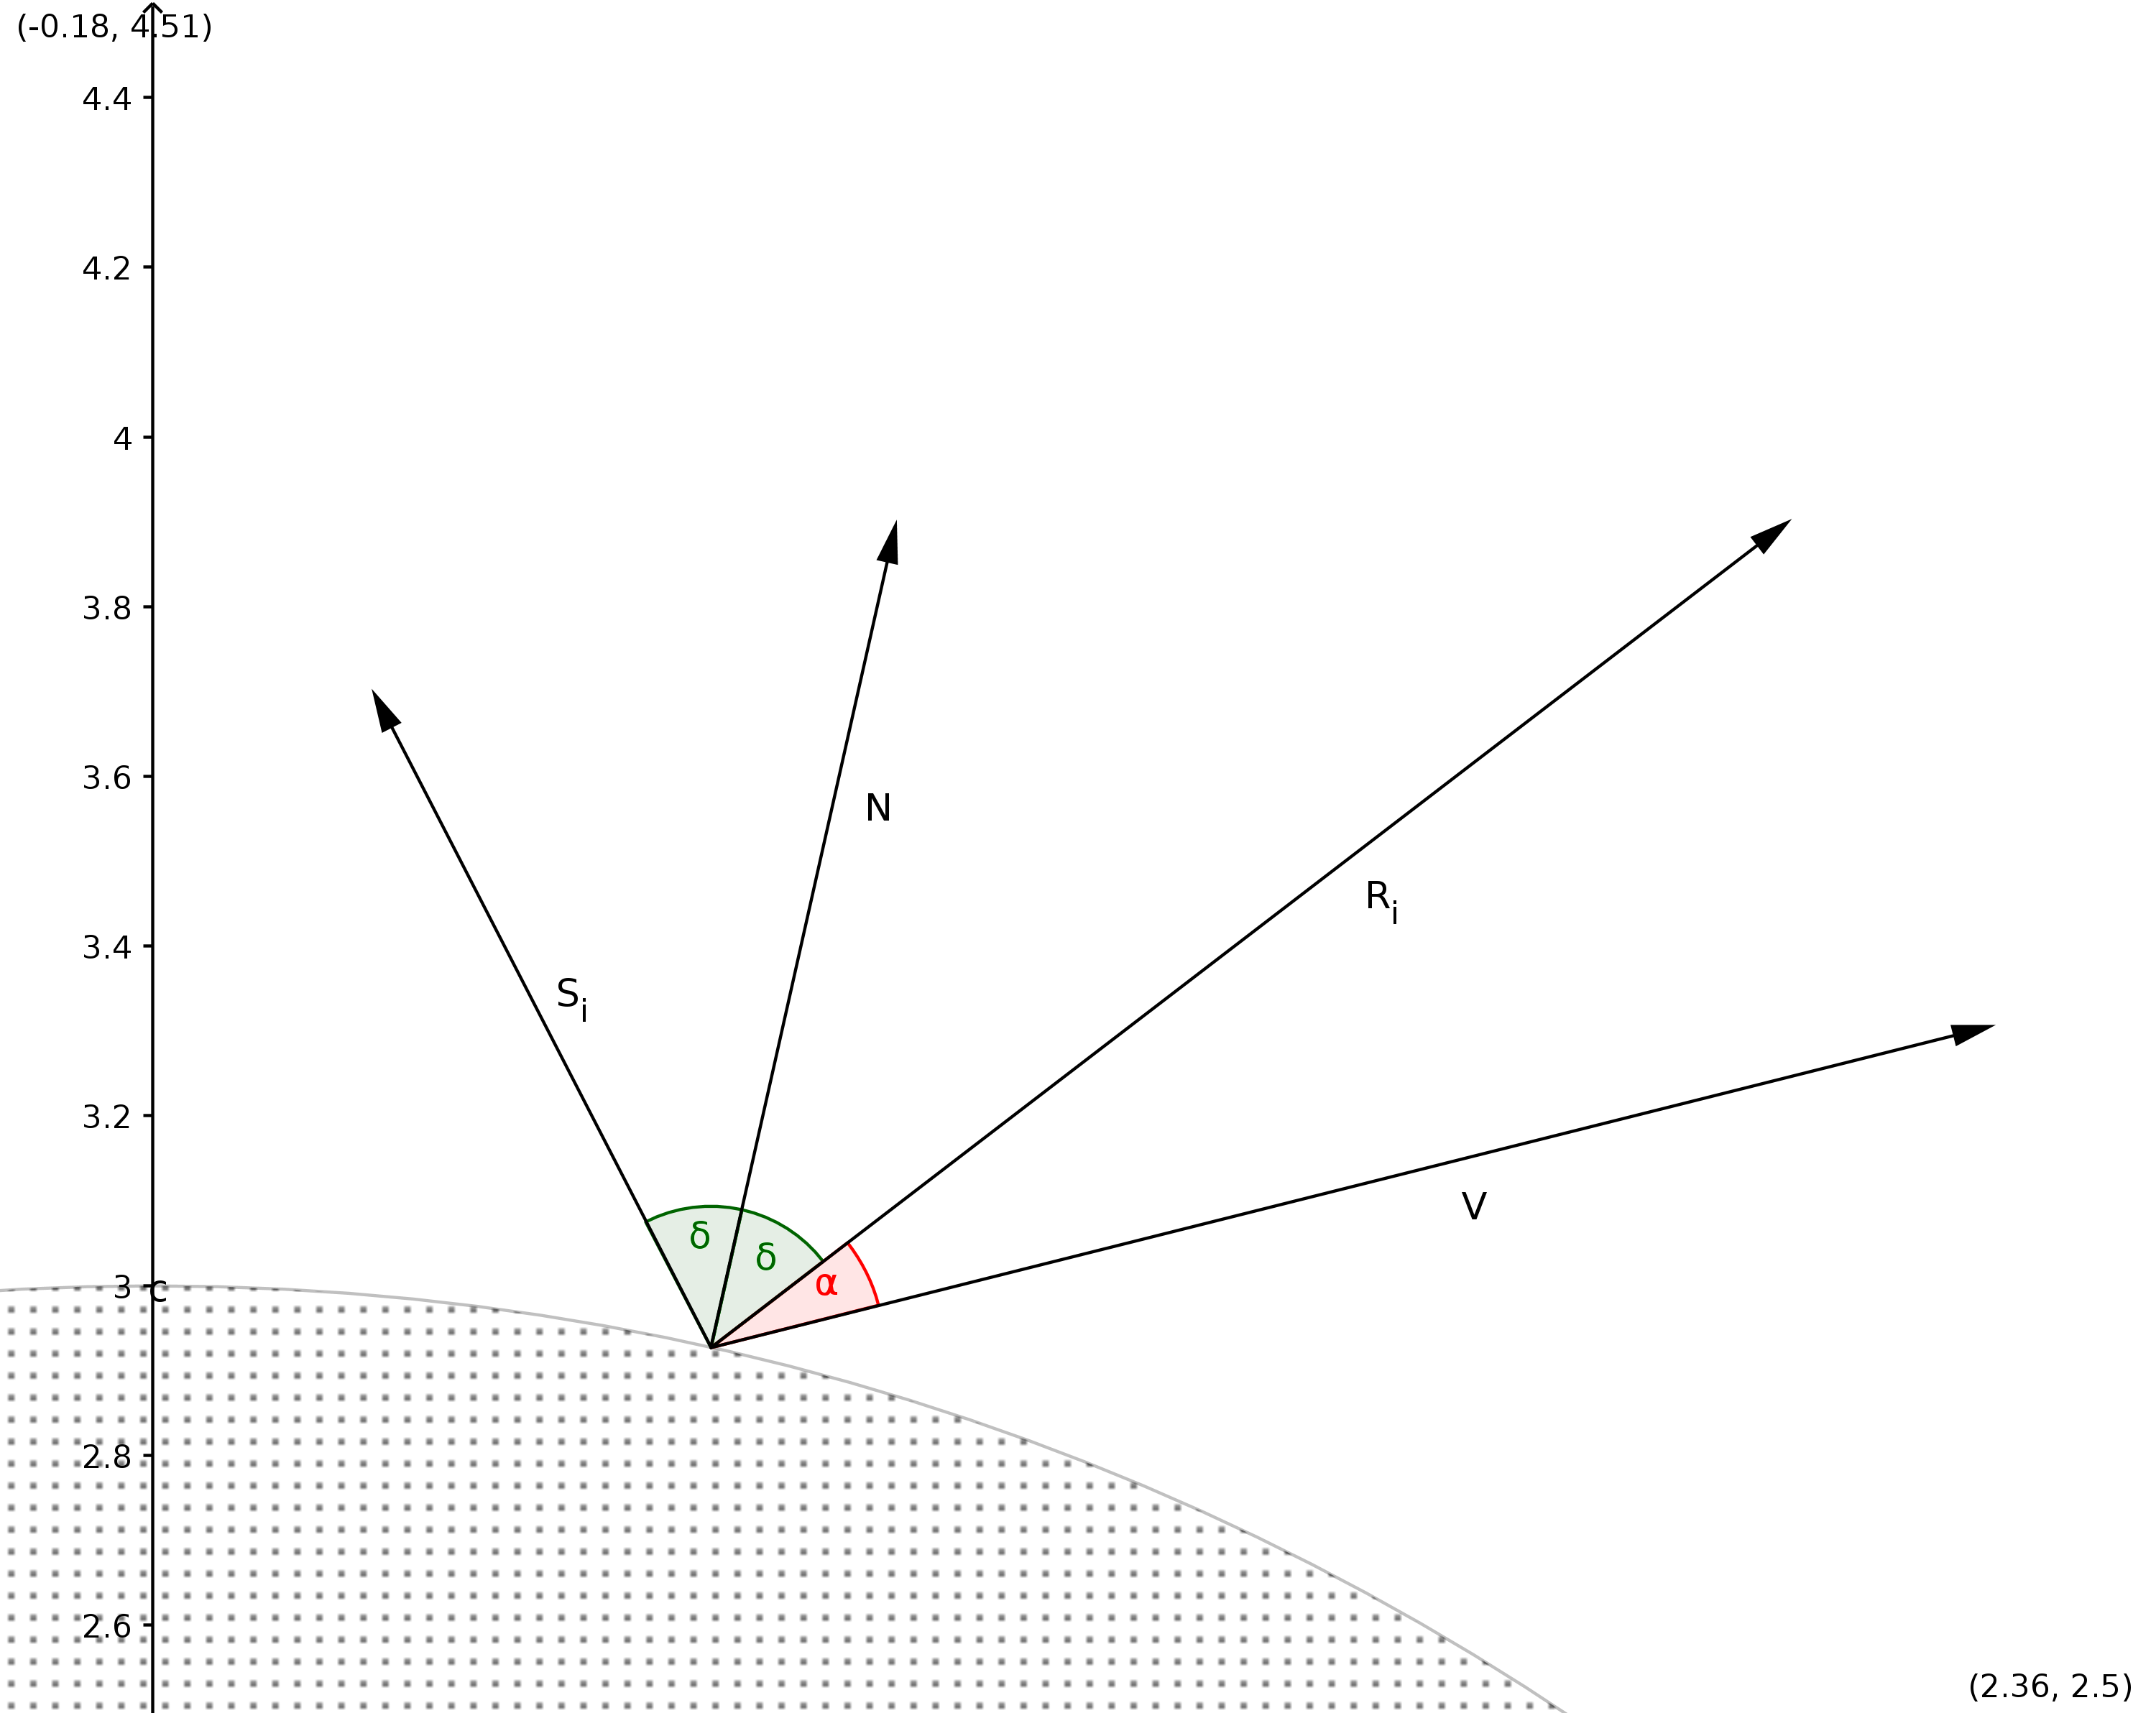
\includegraphics[width=0.4\textwidth]{img/phong_illustration.png}
    \caption{Illustration des Phong-Beleuchtungsmodelles\protect\footnotemark}\label{fig:phong_illustration}
\end{figure}
\footnotetext{Eigene Darstellung mittels Geogebra, angelehnt an~\cite{foley_computer_1996}[Kapitel 16, Seite 731, Abbildung 16.12]}

Es beschreibt die reflektierte (Licht-) Intensität als Zusammensetzung aus der ambienten, der diffusen und der ideal spiegelnden Reflexion einer Oberfläche:

\begin{gather}
    I = I_{\text{ambient}} + I_{\text{diffuse}} + I_{\text{specular}} + I_{\text{emissive}}
\end{gather}

oder mathematisch ausgedrückt:

\begin{gather}
    I(\vv{V}) = k_{a} \cdot L_{a} +
                k_{d} \displaystyle\sum_{i=0}^{n - 1} L_{i} \cdot (\vv{S_{i}} \cdot \vv{N}) +
                k_{s} \displaystyle\sum_{i=0}^{n - 1} L_{i} \cdot {(\vv{R_{i}} \cdot \vv{V})}^{k_{e}}
\end{gather}

wobei gilt:

\begin{itemize}
    \item $I(\vv{V})$:              Die reflektierte (Licht-) Intensität in Richtung des Vektors $\vv{V}$
    \item $n$:                      Anzahl Lichtquellen
    \item $k_{a} \cdot L_{a}$:      Ambiente Komponente des
                                    Beleuchtungsmodelles. Mittels diesem Faktor
                                    wird versucht allem indirekten Licht der
                                    Szene gerecht zu werden.
    \item $k_{d}$:                  Konstante für die diffuse Komponente des
                                    reflektierten Lichtes, basierend auf der
                                    Wellenlänge bzw. Frequenz
    \item $\vv{S_{i}}$:             Richtung, in welcher das Licht der $i$-ten
                                    Lichtquelle ankommt, normalisierter
                                    Einheitsvektor
    \item $\vv{N}$:                 Einheitsnormale der Oberfläche
    \item $k_{s}$:                  Koeffizient der spiegelenden Komponente,
                                    basierend auf der Wellenlänge bzw. Frequenz
    \item $\vv{R_{i}}$:             Richtung, in welcher das Licht der $i$-ten
                                    Lichtquelle reflektiert wird,
                                    normalisierter Einheitsvektor
    \item $\vv{V}$:                 Blickrichtung des Betrachters bzw.\ der
                                    Kamera
    \item $k_{e}$:                  Exponent, welcher von der Rauheit bzw.
                                    Reflektion der Oberfläche abhängt
\end{itemize}


Meist wird der emissive Term bewusst weggelassen, da dieser meist eher für
Spezialeffekte statt für die Beleuchtung ``normaler'' Objekte benutzt wird.

Der reflektive Vektor $R_{i}$ ist gegeben durch

\begin{gather}
    R_{i} = S_{i} + 2(S_{i} \cdot N)N
\end{gather}

Damit die Energieerhaltung gewährleistet ist, muss weiter $k_{d} + k_{s} < 1$
gelten. Der Winkel zwischen $\vv{R}$ und $\vv{V}$ wird mittels $\cos{\alpha}$
ermittelt.


\subsection{Globale Beleuchtungsmodelle}
\label{subsec:global_illumination_models}

Sofern nicht anders vermerkt, basiert der folgende Abschnitt auf~\cite{foley_computer_1996}[S. 775ff]

Globale Beleuchtungsmodelle beschreiben die reflektierte (Licht-) Intensität
eines Punktes aufgrund direkter Lichteinstrahlung durch Lichtquellen sowie
durch alles Licht, welches diesen Punkt nach Reflektion von bzw. Durchdringen
der eigenen oder anderer Oberflächen erreicht.

Bei globalen Beleuchtungsmodellen unterscheidet man zwischen
blickwinkelabhängigen Algorithmen, wie etwa Ray Tracing, und zwischen
blickwinkelunabhängigen Algorithmen, wie etwa Photon Mapping.

Blickwinkelabhängige Algorithmen verwenden eine Diskretisierung der sichtbaren
Fläche bzw. Bildfläche um zu entscheiden, an welchen Punkten, in Blickrichtung
des Betrachters, die Beleuchtungsberechnung durchgeführt werden soll.
Blickwinkelunabhängige Algorithmen hingegen diskretisieren und verarbeiten die
Umgebung um genügend Informationen für die Beleuchtungsberechnung zu haben.
Dies erlaubt ihnen die Beleuchtungsberechnung an einem beliebigen Punkt aus
einer beliebigen Blickrichtung.

Beide Arten von Algorithmen haben jedoch Vor- und Nachteile. So sind
blickwinkelabhängige Algorithmen gut geeignet um Spiegelungen, basierend auf
der Blickrichtung des Betrachtes, zu berechnen, eignen sich aber weniger um
gleichbleibende diffuse Anteile über weiter Flächen eines Bildes zu berechnen.
Bei blickwinkelabhängigen Algorithmen verhält es sich genau umgekehrt.

\subsubsection{Renderinggleichung}
\label{ssubsec:rendering_equation}

Die unter~\ref{subsec:global_illumination_models} genannten Verfahren versuchen
auszudrücken, wie sich Licht von einem Punkt im Raum zu einem anderen bewegt.
Dabei beschreiben sie die Intensität des Lichtes, ausgehend vom ersten Punkt
zum zweiten Punkt. Zusätzlich wird die Intensität des Lichtes, ausgehend von
allen anderen Punkten, welche den ersten Punkt erreichen, und zum zweiten Punkt
emitiert werden, beschrieben.

James (Jim) Kajiya stellte 1986 die so genannte Renderinggleichung auf, welche
genau dieses Verhalten beschreibt~\cite{kajiya_rendering_1986}
und~\cite{foley_computer_1996}:
\begin{equation}
    I(x, x') = g(x, x')[\varepsilon(x, x') + \int\limits_{S}\rho(x, x', x'')I(x', x'')dx'']
\end{equation}
wobei gilt:

\begin{itemize}
    \item $x, x' \text{und } x''$: Punkte in der Umgebung
    \item $ I(x, x')$:            Lichtintensität von Punkt $x'$ nach Punkt $x$
    \item $ g(x, x')$:            Ein auf die Geometrie bezogener Term\\
                                  \hspace*{4mm} $0$:     \hspace*{6mm} $x$ und $x'$ verdecken sich\\
                                  \hspace*{4mm} $1/r^2$: \hspace*{1mm} $x$ und $x'$ sehen sich, wobei $r$ die Distanz zwischen $x$ und $x'$ ist
    \item $\epsilon(x, x')$:      Intensität des Lichtes, welches von $x'$ nach $x$ emitiert wird
    \item $\rho(x, x', x'')$:     Intensität des Lichtes, welches von $x''$
                                  durch die Oberfläche bei $x'$ nach $x$
                                  gestreut wird
    \item $\int\limits_{S}$:      Integral über die Vereinigung aller Flächen,
                                  daher $ S = \bigcup{S_{i}} $\\
                                      Dies bedeutet, dass die Punkte $x$, $x'$
                                      und $x''$ über alle Flächen aller Objekte
                                      der Szene ``streifen''.  Wobei es sich
                                      bei $S_{0}$ um eine zusätzliche Fläche
                                      handelt, welche als Hintergrund verwendet
                                      wird.  $S_{0}$ ist dabei eine Hemisphäre,
                                      welche die gesamte Szene umspannt.
\end{itemize}

\section{Ray Casting und Ray Tracing}
\label{sec:ray_casting_tracing}

\todo[inline]{Expand this section. Add formulas as well as examples.}
\todo[inline]{Punkte mehr ausführen; Integration zeigen mit Diskretition; auch Berechnungen}

Sofern nicht anders vermerkt, basiert der folgende Abschnitt
auf~\cite{hughes_computer_2013}[Kapitel 15, S. 387ff].\\
\\
Um ein Bild möglichst realistisch darzustellen muss berechnet werden, wieviel
Licht zu jedem Pixel der sichtbaren Bildfläche (also dem Betrachter)
transportiert wird. Da Photonen die Energie des Lichtes transportieren, muss
man also das physikalische Verhalten dieser simulieren. Es ist allerdings nicht
möglich \textit{alle} Photonen zu simulieren, da der Aufwand schlicht zu gross
wäre. Daher macht es Sinn nur einige Photonen (exemplarisch) zu betrachten und
dann eine Abschätzung des gesamten Lichtes vorzunehmen.\\

\subsection{Ray Casting}
\label{subsec:ray_casting}

Bei \textbf{Ray Casting} handlt es sich grundsätzlich um eine Strategie zur
Simulation, wieviel Licht anhand eines (Licht-) Strahles zu der sichtbaren
Bildfläche (also dem Betrachter) transportiert wird.

\begin{figure}[H]
    \centering \rotatebox{0}{\scalebox{0.3}[0.3]{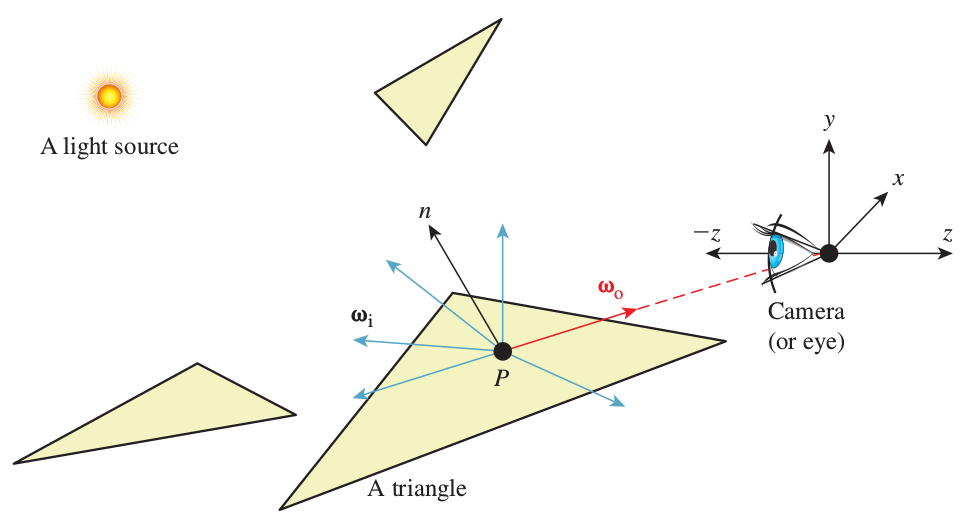
\includegraphics{img/ray_tracing_01.png}}}
    \caption{Punkt $P$ auf einer Oberfläche eines Dreieckes, welcher für die Kamera bzw.\ den Betrachter sichtbar ist.
        Der Betrachter nimmt dabei das Licht, welches aus verschiedenen Richtungen $\omega_{i}$ kommt, über den Punkt $P$ in Richtung $\omega_{0}$ wahr.\label{fig:ray_casting:basics}\protect\footnotemark}
\end{figure}
\footnotetext{Darstellung von~\cite{hughes_computer_2013}[Kapitel 15, Seite 389, Abbildung 15.1]}

Wie in Abbildung~\ref{fig:ray_casting:basics} ersichtlich, gelangt Licht aus vielen Richtungen durch den Punkt $P$ zu dem Betrachter. Dies beinhaltet auch die Möglichkeit, dass
Licht nicht nur von einer Lichtquelle aus, sondern von vielen Lichtquellen aus via $P$ zum Betrachter gelangt. Weiter ist es möglich, dass Licht zuvor an anderen Punkten gestreut
und/oder gespiegelt und erst dann via $P$ zum Betrachter gelangte.\\
\\
Dies führt zu den folgenden Schlussfolgerungen:
\begin{itemize}
    \item Es müssen alle möglichen Richtungen, aus denen Licht kommen könnte,
        an Punkt $P$ untersucht werden.
    \item Da, bedingt durch technische Limitierungen, nur diskretes Abtasten
        möglich ist, müssen die Richtungen auf eine endliche Anzahl beschränkt
        werden, was zu Abtastfehlern führen kann.
\end{itemize}
Um die Abtastfehler zu minieren, können die Richtungen des Abtasten anhand der Lichtquellen priorisiert werden.

\newpage{}

Ein möglicher Algorithmus, wie solch ein Verfahren umgesetzt werden kann,
findet sich in~\ref{fig:ray_casting:high_level}.

\begin{lstlisting}[language=Python,caption={Eine abstrakte Umsetzung des Ray
        Castings\protect\footnotemark.},label={fig:ray_casting:high_level},captionpos=b,emph={ray_cast}]
def ray_cast():
    # "pixels" is a list of all pixels of the image plane
    for pixel in pixels:
        # Save all intersections for given pixel
        intersections = []

        # Returns the ray passing through the given
        # pixel from the eye
        ray = ray_at_pixel(pixel)

        # "scene_triangles" is a list of all triangles
        # coming from meshes contained in the scene to render
        for triangle in scene_triangles:
            p   = intersect(ray, triangle)
            sum = 0

            for light in incoming_lights_at_p:
                sum = sum + l.value
            end

            if is_smallest_intersection(p, intersections):
                pixel = sum
            intersections.append(p)
\end{lstlisting}
\footnotetext{Algorithmus in Pseudocode gemäss~\cite{hughes_computer_2013}[Kapitel 15, Seite 391, Auflistung 15.2]}

Das Verfahren wurde erstmals 1968 in~\cite{appel_techniques_1968} vorgeschlagen
und auch 1968 von der Matthematical Applications Group Inc.\
in~\cite{arlington_mathematical_applications_group_inc_afips_1968} erfolgreich umgesetzt.

\subsection{Ray Tracing}
\label{subsec:ray_tracing}

Bei dem heute als Ray Tracing bekannten Verfahren, handelt es sich um eine
verbesserte Version des unter~\ref{subsec:ray_casting} genannten Ray Casting
Verfahrens. Dieses wurde im Juni 1980 durch~\cite{whitted_improved_1980}[S.
345] verbessert.

So schlägt~\cite{whitted_improved_1980} vor, dass die Berechnung der
Sichtbarkeit (von Objekten) nicht bei dem nähesten gefundenen Schnittpunkt
abgebrochen wird, sondern dass jedes Auftreffen eines (Licht-) Strahles mehr
(Licht-) Strahlen durch Transmission bzw. Reflektion sowie in Richtung jeder
Lichtquelle gesendet werden. Dieser Prozess wird so lange wiederholt, bis
keiner der neu generierten (Licht-) Strahlen mehr auf ein Objekt
trifft~\cite{whitted_improved_1980}[S.  345].\\
Es handelt sich dabei also um ein rekursives Verfahren und wird daher
teilweise auch rekurisves Ray Tracing genannt.

\begin{figure}[H]
    \centering
    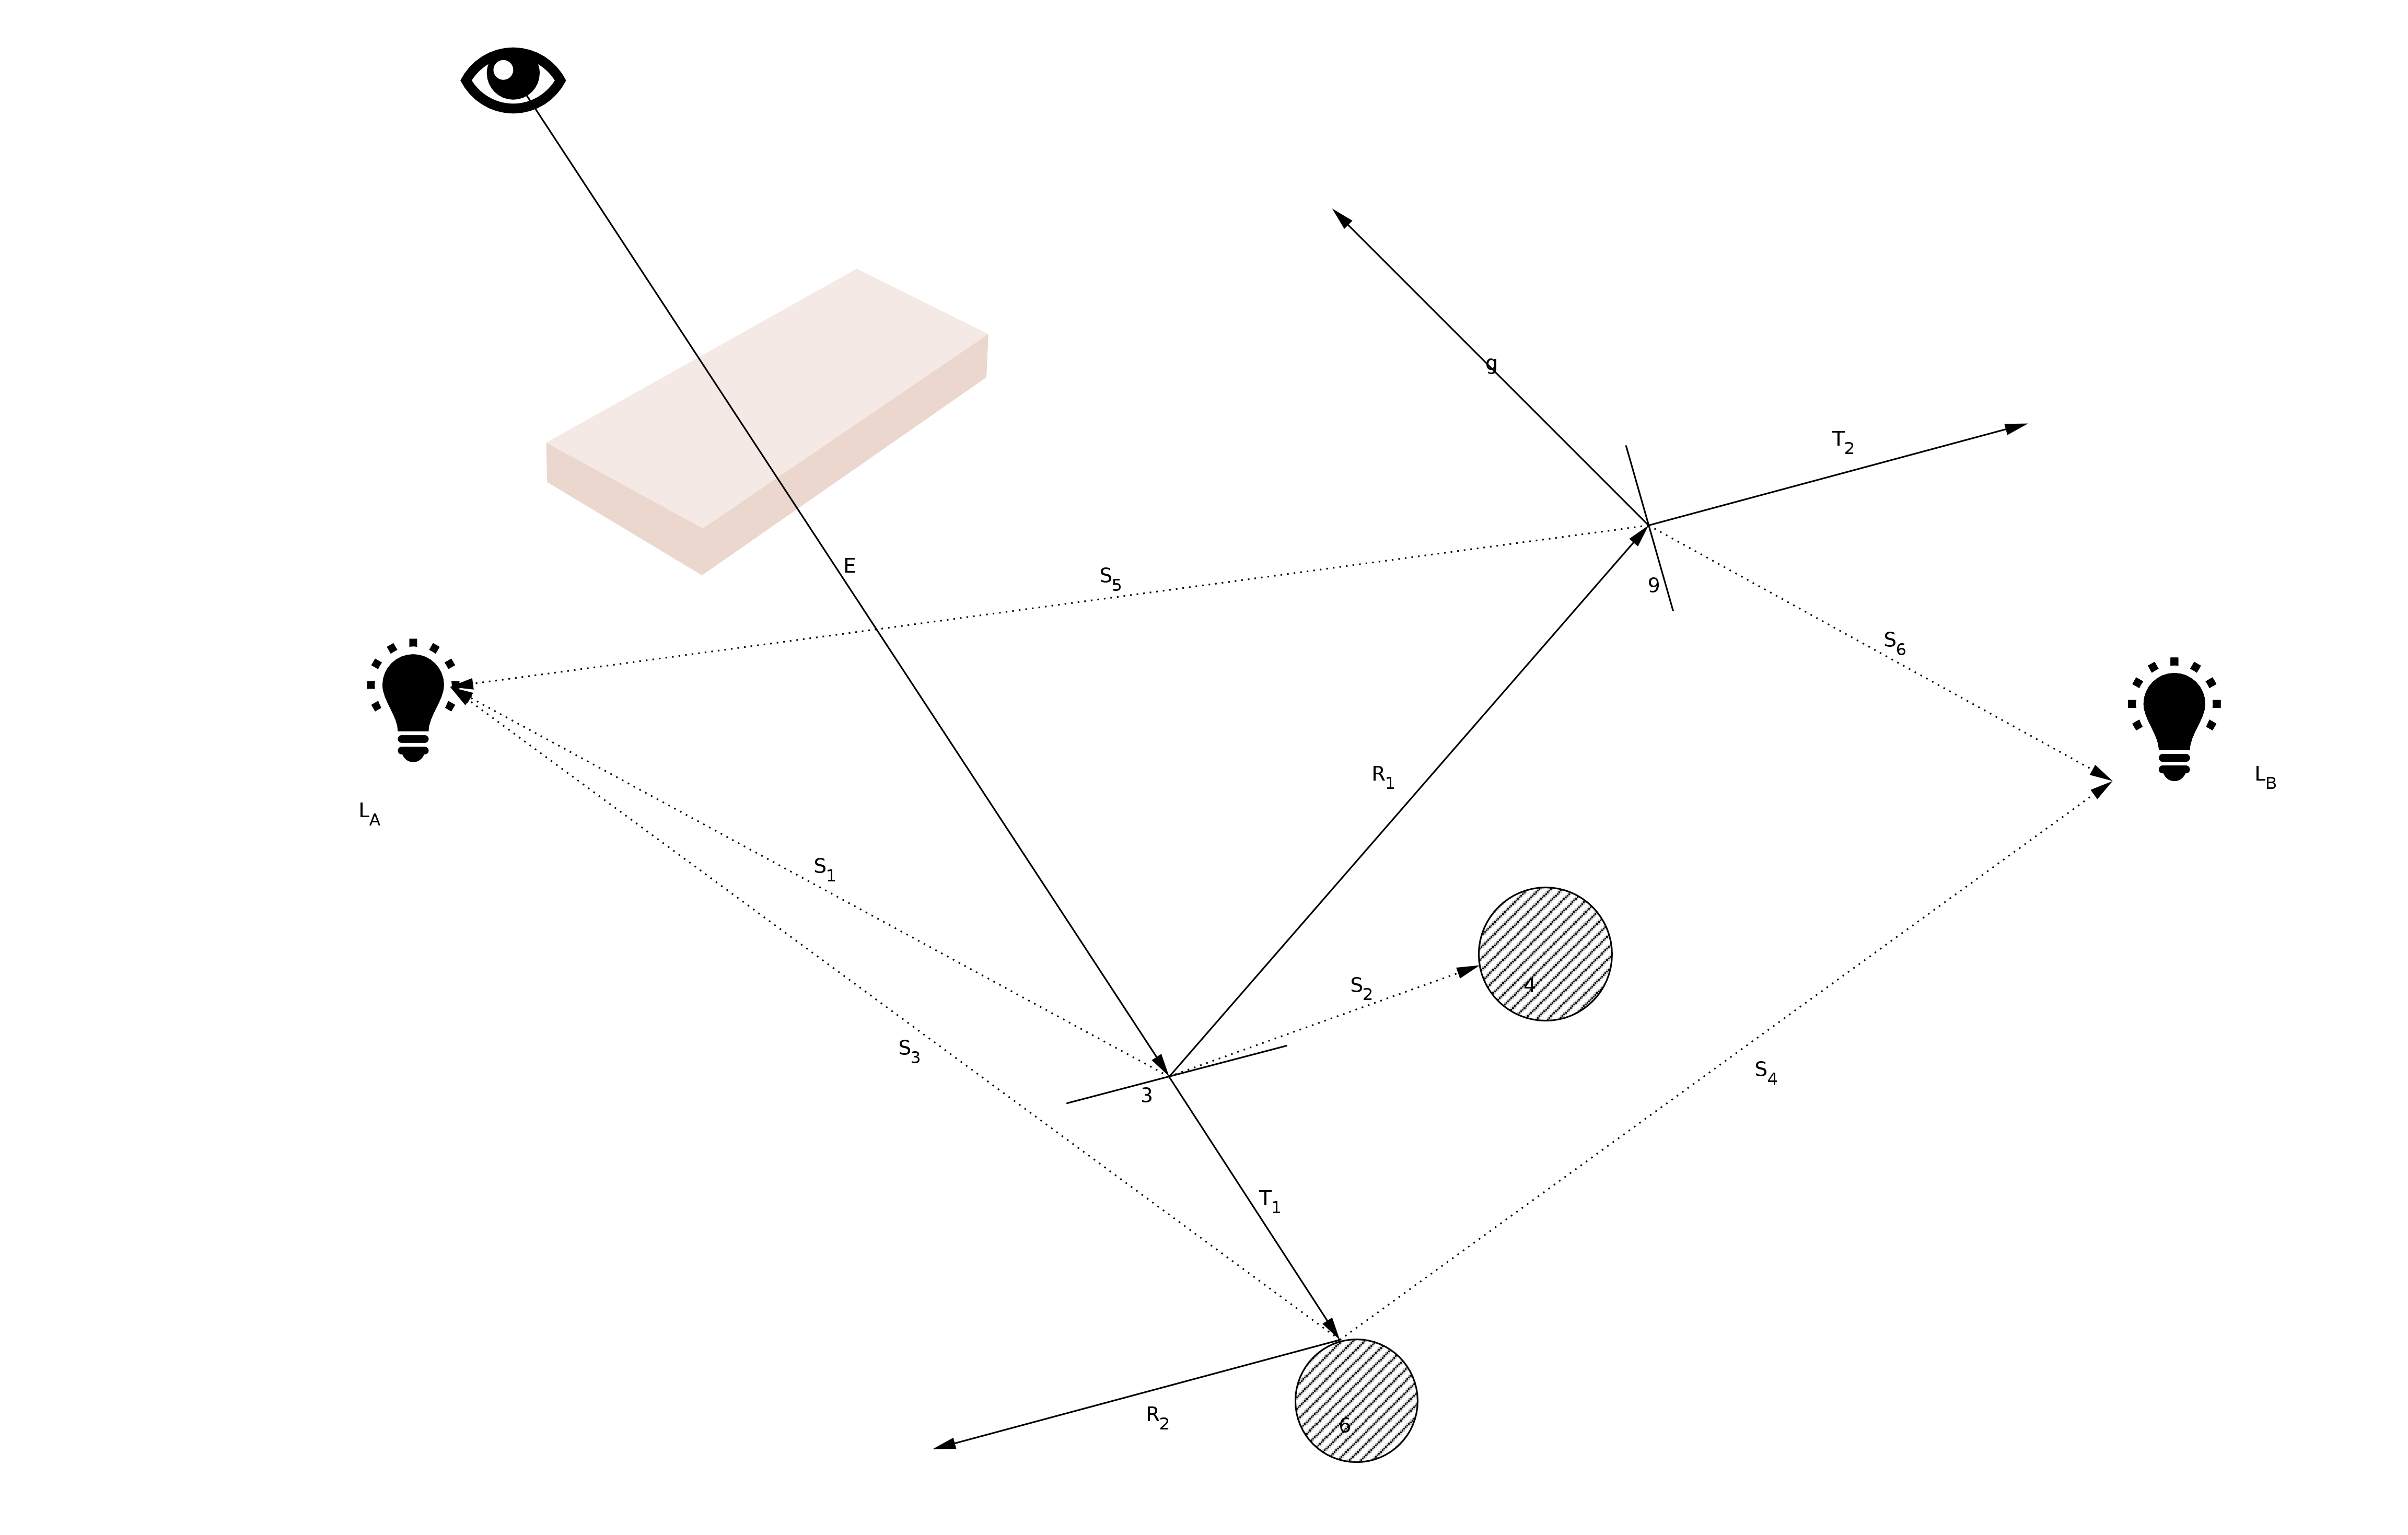
\includegraphics[width=1.0\textwidth]{img/ray_tracing_illustration.png}
    \caption{Illustration des Ray Tracing Verfahrens\protect\footnotemark}\label{fig:ray_tracing_illustration}
\end{figure}
\footnotetext{Eigene Darstellung mittels Geogebra, angelehnt an~\cite{glassner_introduction_1989}[Kapitel 2, Seite 16, Abbildung 11; Piktogramm Auge erstellt von ``Icomoon'' auf www.flaticon.com; Piktogramm Glühbirne erstellt von ``Simpleicon'' auf www.flaticon.com;]}
\todo[inline]{Explain illustration~\ref{fig:ray_tracing_illustration}}
\todo[inline]{Explain transmission and refraction}
\todo[inline]{Add an (sphere) example, explain basic terminology (illum.\ and
    shadow rays, aliasing and so on)}

% -*- coding: UTF-8 -*-
% vim: autoindent expandtab tabstop=4 sw=4 sts=4 filetype=tex
% chktex-file 27 - disable warning about missing include files

\section{Modelle zur Schattierung (shading models)}
\label{sec:shading}

% * Lighting model at each vertex, e.g. Lambert
% * Shading: Compute the color of interior points between vertices
% * Example image of mesh (vertices)

Sofern nicht anders vermerkt, basieren die nachfolgenden Abschnitte
auf~\cite{foley_computer_1996}[S. 734–739].

Bei der Anwendung von Modellen zur Schattierung (shading models) geht es
grundsätzlich darum die emitierte Lichtintensität bzw.\ die Farbe einer
Oberfläche an einem bestimmten Punkt zu berechnen. Es wäre naheliegend
dies für jeden sichtbaren Punkt der Oberfläche zu berechnen, dies ist
jedoch häufig viel zu aufwändig. Viele Modelle zur Schattierung
berechnen daher die Licht- bzw. Farbintensität nur an gewissen
Schlüsselpunkten und wenden dann vereinfachte Modelle zur Berechnung an
um so Rechenzeit zu sparen.

Als Beispiel zur Anwendung der Schattierungsmodelle wird nachfolgend
angenommen, dass mittels einem Beleuchtungsmodell an jedem Eckpunkt einer
Oberfläche (Polygon) die Farbe berechnet wird. Als Beispiel dienen hier die
Eckpunkte $\bm{V}_{1}$, $\bm{V}_{2}$, $\bm{V}_{3}$ und $\bm{V}_{4}$.

Um einen Farbintensitätswert für einen Eckpunkt $\bm{V}_{1}$ zu berechnen, wird der
Normalenvektor des Eckpunktes (vertex normal) benötigt. Es handelt sich dabei
um den Normalenvektor der Oberfläche an der Position des Eckpunktes $\bm{V}_{1}$.

\todo[inline]{Translate/cite}
Modern shaders are really graphics programs rather than being restricted to
computing colors of points. There are geometry shaders, which can alter the
list of triangles to be processed in subsequent stages, and tessellation
shaders, which take high-level descriptions of surfaces and produce triangle
lists from them; an example is a subdivision surface shader, which might take
as input the vertices and mesh structure of a subdivision surface’s control
mesh, and produce as output a collection of tiny triangles that form a good
approximation of the limit surface. There are also vertex shaders that serve
only to transform the vertex locations, and generally have nothing to do with
eventual color.

\subsection{Flat shading --- per vertex lighting}
\label{subsec:flat_shading}

% * Calculate normal for each vertice by averaging line-segment normals, e.g.
%   (normal(V1V2) + normal(V3V4)) / 2 to determine per vertex color
%   * Image of calculated normals: line-segment (given through mesh) and vertex
% * One color per face determined by vertex' color

Bei Flat-Shading wird pro Oberfläche (Polygon) ein Eckpunkt $\bm{V}_{1}$ dieser als
farb- bzw.\ intensitätgebender Schlüsselpunkt bestimmt. Danach wird die Farbe
des Punktes als Farbe für die Oberfläche genommen.

Diese Annahme ist unter den folgenden Voraussetzungen gültig:
\begin{enumerate}
    \item{Die zugrundeliegende Lichtquelle befindet sich unendlich weit
            entfernt, so dass der Winkel zwischen dem
            Normalenvektor der Oberfläche und der Lichtquelle
            $\bm{n}\cdot{}\bm{l}$ für die gesamte Oberfläche konstant ist.}
    \item{Der Betrachter sich unendlich weit entfernt von der Oberfläche
            befindet, so dass der Winkel zwischen dem Normalenvektor der
            Oberfläche und dem Betrachter $\bm{n}\cdot{}\bm{v}$ für die
            gesamte Oberfläche konstant ist.}
    \item{Das Polygon ist eine effektive Repräsentation der Oberfläche
            und nicht nur eine Näherung einer runden Oberfläche.}
\end{enumerate}

Ist eine der ersten beiden Annahmen falsch, so muss für den Vektor der
Lichtquelle $\bm{l}$ bzw.\ den Vektor des Betrachters $\bm{v}$ ein
konstanter Wert berechnet werden.~\citeauthor{foley_computer_1996} gibt
hier als Beispiele das Zentrum des Polygones oder den ersten Eckpunkt
des Polygones an.

\subsection{Gouraud shading --- face interpolated lighting}
\label{subsec:gouraud_shading}

Bei Gouraud-Shading handelt es sich um ein Shading-Verfahren, welches die
Farbintensitätswerte der Eckpunkte von Oberflächen eines Meshes interpoloiert.

Um den Farbintensitätswert eines Eckpunktes von Oberflächen  zu berechnen,
schlägt Gouraud die Berechnung des Durchschnittswertes der Oberflächennormalen
zweier adjazenter Liniensegmente (im 2D-Raum) bzw.\  aller adjazenter Dreiecke
(im 3D-Raum) vor.

\todo[inline]{Image explaining average calculation}

Die Berechnung des Normalenvektors eines Eckpunktes via Durchschnittswert ist
üblicherweise eine genügend gute Näherung der Oberflächennormale der
eigentlichen Oberfläche. Die Präzision hängt dabei aber klar von der
Granularität des Modelles (mesh) ab.

\subsection{Phong shading --- normal interpolated lighting}
\label{subsec:phong_shading}

\todo[inline]{Translate/cite}

Phong shading improves upon Gouraud shading and provides a better approximation
of the shading of a smooth surface. Phong shading assumes a smoothly varying
surface normal vector. The Phong interpolation method works better than Gouraud
shading when applied to a reflection model that has small specular highlights
such as the Phong reflection model.

Unlike Gouraud shading, which interpolates colors across polygons, in Phong
shading a normal vector is linearly interpolated across the surface of the
polygon from the polygon's vertex normals. The surface normal is interpolated
and normalized at each pixel and then used in a reflection model, e.g.\ the
Phong reflection model, to obtain the final pixel color. Phong shading is more
computationally expensive than Gouraud shading since the reflection model must
be computed at each pixel instead of at each vertex.

